\documentclass[aspectratio=169]{beamer}

% ── Theme ──────────────────────────────────────────────────────────────────────
\usetheme{Madrid}
\usecolortheme{seahorse}
\usefonttheme{professionalfonts}

% ── Packages ───────────────────────────────────────────────────────────────────
\usepackage{amsmath,amssymb}
\usepackage{booktabs}
\usepackage{array}
\usepackage{xcolor}
\usepackage{tikz}
\usetikzlibrary{shapes.geometric, arrows.meta, positioning, fit, backgrounds}
\usepackage{listings}
\usepackage{microtype}
\usepackage{graphicx}

% ── Color palette ──────────────────────────────────────────────────────────────
\definecolor{ppoBlue}{RGB}{41,128,185}
\definecolor{cfOrange}{RGB}{211,84,0}
\definecolor{greedyGreen}{RGB}{39,174,96}
\definecolor{darkGray}{RGB}{44,62,80}
\definecolor{lightBg}{RGB}{236,240,241}
\definecolor{accentRed}{RGB}{192,57,43}

\setbeamercolor{palette primary}{bg=darkGray,fg=white}
\setbeamercolor{palette secondary}{bg=ppoBlue,fg=white}
\setbeamercolor{palette tertiary}{bg=ppoBlue!80,fg=white}
\setbeamercolor{frametitle}{bg=darkGray,fg=white}
\setbeamercolor{title}{fg=white}
\setbeamercolor{block title}{bg=ppoBlue,fg=white}
\setbeamercolor{block body}{bg=lightBg}
\setbeamercolor{alerted text}{fg=accentRed}
\setbeamertemplate{navigation symbols}{}
\setbeamertemplate{footline}[frame number]

% ── Code listings ──────────────────────────────────────────────────────────────
\lstset{
  basicstyle=\ttfamily\scriptsize,
  keywordstyle=\color{ppoBlue}\bfseries,
  commentstyle=\color{gray}\itshape,
  stringstyle=\color{accentRed},
  backgroundcolor=\color{lightBg},
  frame=single,
  framerule=0.4pt,
  rulecolor=\color{ppoBlue!40},
  breaklines=true,
}

% ── Metadata ───────────────────────────────────────────────────────────────────
\title[RL-Based Dynamic Request Batching]
      {\textbf{Reinforcement Learning for\\Dynamic Request Batching}\\
       \small on GPU Inference Servers}
\author{Sudarshan Sudhakar}
\institute[]{Semester 6 RL Project}
\date{May 2026}

% ══════════════════════════════════════════════════════════════════════════════
\begin{document}
% ══════════════════════════════════════════════════════════════════════════════

% ── Title slide ───────────────────────────────────────────────────────────────
\begin{frame}[plain]
  \begin{tikzpicture}[remember picture, overlay]
    \fill[darkGray] (current page.north west) rectangle (current page.south east);
    \fill[ppoBlue!60] (current page.north west) -- ++(0,-2.5) -- ++(16,0) -- cycle;
  \end{tikzpicture}
  \vspace{0.8cm}
  \titlepage
\end{frame}

% ── Slide 1: Motivation ────────────────────────────────────────────────────────
\begin{frame}{Motivation: The Batching Dilemma}
  \begin{columns}[T]
    \column{0.52\textwidth}
      \begin{block}{The Setting}
        A GPU inference node receives \textbf{2\,000 req/s} (peak: 5\,000 req/s).
        Every \textbf{10\,ms} a batching layer must decide:\\[4pt]
        \quad \textcolor{ppoBlue}{\textbf{Wait}} — accumulate more requests\\
        \quad \textcolor{cfOrange}{\textbf{Serve}} — dispatch the batch now
      \end{block}
      \vspace{6pt}
      \begin{alertblock}{The Problem}
        \begin{itemize}
          \item \textbf{Too aggressive}: tiny batches, wasted GPU kernel launches
          \item \textbf{Too conservative}: long queues, SLA violations
          \item Fixed thresholds cannot adapt to \textbf{traffic dynamics}
        \end{itemize}
      \end{alertblock}

    \column{0.44\textwidth}
      \begin{block}{GPU Efficiency vs.\ Latency}
        \vspace{4pt}
        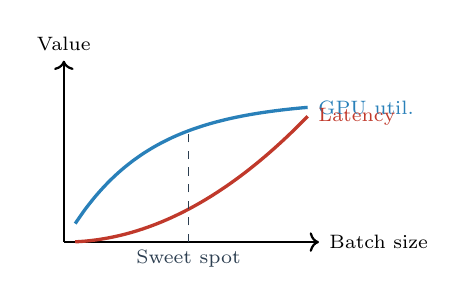
\begin{tikzpicture}[scale=0.72]
          % Axes
          \draw[->,thick] (0,0) -- (4.5,0) node[right]{\scriptsize Batch size};
          \draw[->,thick] (0,0) -- (0,3.2) node[above]{\scriptsize Value};
          % Efficiency curve
          \draw[ppoBlue,very thick,domain=0.2:4.3,smooth]
            plot(\x,{2.5*(1-exp(-0.7*\x))}) node[right]{\scriptsize\color{ppoBlue}GPU util.};
          % Latency curve
          \draw[accentRed,very thick,domain=0.2:4.3,smooth]
            plot(\x,{0.12*\x*\x}) node[right]{\scriptsize\color{accentRed}Latency};
          % Sweet spot
          \draw[dashed,darkGray] (2.2,0) -- (2.2,2.05);
          \node[darkGray,font=\scriptsize] at (2.2,-0.3) {Sweet spot};
        \end{tikzpicture}
      \end{block}
  \end{columns}
\end{frame}

% ── Slide 2: Problem Statement ────────────────────────────────────────────────
\begin{frame}{Problem Statement}
  \begin{columns}[T]
    \column{0.48\textwidth}
      \begin{block}{Formal Objective}
        Learn a policy $\pi : \mathcal{S} \to \{0,1\}$ that maximises
        cumulative reward subject to:
        \begin{equation*}
          \text{wait}_{i} + t_{\text{proc}}(n) \;\leq\; \text{SLA}_{500}
          \quad \forall\, \text{request}\; i
        \end{equation*}
        where $t_{\text{proc}}(n) = 8 + 0.12n$ ms (GPU model).
      \end{block}
      \vspace{4pt}
      \begin{block}{Why RL?}
        \begin{itemize}
          \item State is \textbf{high-dimensional and continuous}
          \item Optimal threshold \textbf{varies with traffic rate}, time-of-day,
                queue age — cannot be hand-tuned
          \item No closed-form optimal policy exists
        \end{itemize}
      \end{block}

    \column{0.48\textwidth}
      \begin{exampleblock}{Key Numbers}
        \renewcommand{\arraystretch}{1.3}
        \begin{tabular}{ll}
          \toprule
          \textbf{Parameter} & \textbf{Value} \\
          \midrule
          Arrival rate & 2\,000 req/s (base) \\
          Peak rate & 5\,000 req/s \\
          Decision interval & 10\,ms (100\,Hz) \\
          SLA budget & 500\,ms total latency \\
          Max batch & 512 requests \\
          Min batch & 8 requests \\
          GPU base overhead & 8.0\,ms \\
          GPU per-request & 0.12\,ms \\
          Episode length & 60\,s simulated \\
          \bottomrule
        \end{tabular}
      \end{exampleblock}
  \end{columns}
\end{frame}

% ── Slide 3: MDP Formulation ──────────────────────────────────────────────────
\begin{frame}{MDP Formulation}
  \begin{columns}[T]
    \column{0.50\textwidth}
      \begin{block}{State Space — 8-dimensional Box}
        \renewcommand{\arraystretch}{1.2}
        \begin{tabular}{@{}cl@{}}
          \toprule
          \textbf{Dim} & \textbf{Feature} \\
          \midrule
          0 & \texttt{pending\_requests} $\in [0,512]$ \\
          1 & \texttt{oldest\_wait\_ms} $\in [0,1000]$ \\
          2 & \texttt{request\_rate} (EMA, req/s) \\
          3 & \texttt{since\_serve\_ms} \\
          4 & \texttt{batch\_fill\_ratio} $\in [0,1]$ \\
          5 & \texttt{time\_of\_day} $\in [0,24)$ \\
          6 & \texttt{urgency\_ratio}$^*$ $\in [0,3]$ \\
          7 & \texttt{rate\_trend} $\in [-1,1]$ \\
          \bottomrule
        \end{tabular}\\[4pt]
        \scriptsize $^*$ urgency $= \frac{\text{oldest\_wait}}{\text{SLA} - t_\text{proc}(n)}$;
        value $>1$ signals imminent SLA breach.
      \end{block}
      \begin{block}{Action Space}
        $\mathcal{A} = \{0\,(\text{Wait}),\; 1\,(\text{Serve})\}$
      \end{block}

    \column{0.46\textwidth}
      \begin{block}{Reward Function}
        \textbf{Serve action:}
        \begin{align*}
          r &= \alpha \cdot n - \beta \cdot w_{\max}\\
            &\quad - c_{\text{dispatch}}\\
            &\quad - \lambda \textstyle\sum_i \max(0,\, l_i - \text{SLA})
        \end{align*}
        \textbf{Wait action:}
        \begin{align*}
          r &= -\beta \cdot w_{\max} - \mathbf{1}_{q=0}\cdot c_{\text{idle}}
        \end{align*}
        \vspace{4pt}
        \renewcommand{\arraystretch}{1.15}
        \begin{tabular}{@{}ll@{}}
          $\alpha=1.0$ & revenue per request \\
          $\beta=0.003$ & urgency weight \\
          $c_{\text{dispatch}}=5.0$ & fixed GPU overhead \\
          $\lambda=0.3$ & SLA violation penalty \\
        \end{tabular}\\[4pt]
        \footnotesize Key: $c_\text{dispatch}$ forces the agent to
        accumulate $\geq$5 requests before serving is profitable.
      \end{block}
  \end{columns}
\end{frame}

% ── Slide 4: Algorithms Compared ─────────────────────────────────────────────
\begin{frame}{Algorithms: Four Approaches Compared}
  \begin{columns}[T]
    \column{0.48\textwidth}
      \begin{block}{\textcolor{ppoBlue}{PPO — Proximal Policy Optimization}}
        On-policy actor-critic with clipped surrogate objective:
        \begin{equation*}
          L^{\text{CLIP}} = \mathbb{E}\!\left[\min\!\left(r_t A_t,\;
          \text{clip}(r_t, 1\!\pm\!\epsilon) A_t\right)\right]
        \end{equation*}
        \begin{itemize}\itemsep2pt
          \item $\epsilon=0.2$ clip, GAE $\lambda=0.95$, entropy $0.005$
          \item VecNormalize on all 8 obs dims
          \item 4 parallel envs, 1\,M steps, $[128,128]$ MLP
        \end{itemize}
      \end{block}
      \vspace{4pt}
      \begin{block}{\textcolor{cfOrange}{D3QN — Dueling Double DQN + PER}}
        \begin{itemize}\itemsep2pt
          \item Dueling streams: $Q = V(s) + A(s,a) - \overline{A}$
          \item Double DQN: decoupled target evaluation
          \item Prioritized Replay ($\alpha=0.6$, $\beta$: 0.4$\to$1.0)
          \item 3-step returns, $\varepsilon$-greedy decay to 0.02
        \end{itemize}
      \end{block}

    \column{0.48\textwidth}
      \begin{block}{\textcolor{greedyGreen}{Recurrent PPO (R-PPO)}}
        \begin{itemize}\itemsep2pt
          \item LSTM layer before policy/value heads
          \item Captures temporal correlations explicitly
          \item Higher compute cost; used as ablation baseline
        \end{itemize}
      \end{block}
      \vspace{4pt}
      \begin{block}{\textcolor{darkGray}{Discrete SAC}}
        \begin{itemize}\itemsep2pt
          \item Off-policy, maximum-entropy framework
          \item Automatic entropy tuning: $H_\text{target} = 0.5\ln(2)$
          \item Soft Q-functions with target smoothing $\tau=0.005$
        \end{itemize}
      \end{block}
      \vspace{6pt}
      \begin{alertblock}{Final Model: \textbf{PPO}}
        Best convergence speed, stability, and deployment simplicity.
        Stateless inference — no LSTM hidden state to manage.
      \end{alertblock}
  \end{columns}
\end{frame}

% ── Slide 5: Architecture ─────────────────────────────────────────────────────
\begin{frame}{System Architecture}
  \begin{center}
  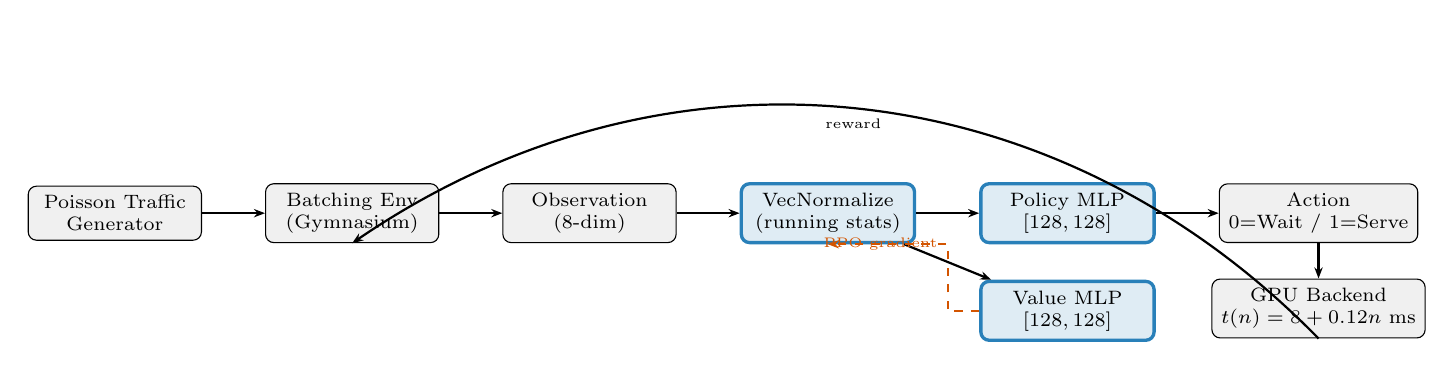
\begin{tikzpicture}[
    node distance=0.55cm and 0.9cm,
    box/.style={rectangle, rounded corners=3pt, draw, minimum width=2.2cm,
                minimum height=0.65cm, font=\scriptsize, align=center},
    boldbox/.style={box, very thick, fill=ppoBlue!15, draw=ppoBlue},
    graybox/.style={box, fill=gray!12},
    arr/.style={-{Stealth[length=4pt]}, thick},
  ]
    % Traffic
    \node[graybox] (traf) {Poisson Traffic\\Generator};
    \node[graybox, right=0.8cm of traf] (env) {Batching Env\\(Gymnasium)};
    \node[graybox, right=0.8cm of env]  (obs)  {Observation\\(8-dim)};

    % PPO
    \node[boldbox, right=0.8cm of obs]  (norm) {VecNormalize\\(running stats)};
    \node[boldbox, right=0.8cm of norm] (pol) {Policy MLP\\$[128,128]$};
    \node[boldbox, below=0.45cm of pol] (val) {Value MLP\\$[128,128]$};

    % Action
    \node[graybox, right=0.8cm of pol]  (act)  {Action\\0=Wait / 1=Serve};
    \node[graybox, below=0.45cm of act] (gpu)  {GPU Backend\\$t(n)=8+0.12n$ ms};

    % Arrows
    \draw[arr] (traf) -- (env);
    \draw[arr] (env)  -- (obs);
    \draw[arr] (obs)  -- (norm);
    \draw[arr] (norm) -- (pol);
    \draw[arr] (norm) -- (val);
    \draw[arr] (pol)  -- (act);
    \draw[arr] (act)  -- (gpu);
    \draw[arr,bend right=40] (gpu.south) to node[below,font=\tiny]{reward} (env.south);

    % Gradient
    \draw[arr,dashed,cfOrange] (val.west) -- ++(-0.4,0) |-
      node[left,font=\tiny,cfOrange]{PPO gradient} (norm.south);
  \end{tikzpicture}
  \end{center}

  \vspace{4pt}
  \begin{columns}[T]
    \column{0.32\textwidth}
      \begin{block}{\scriptsize Environment}
        \scriptsize Simulates 60\,s of traffic per episode.
        Poisson arrivals with time-of-day multipliers
        ($\times 2.5$ peak, $\times 0.2$ off-peak).
        Queue capped at 512.
      \end{block}
    \column{0.32\textwidth}
      \begin{block}{\scriptsize Training}
        \scriptsize 4 parallel envs via \texttt{SubprocVecEnv}.
        VecNormalize runs online — critical because features span
        [0,512] to [0,1].
        Best checkpoint saved every 20\,k steps.
      \end{block}
    \column{0.32\textwidth}
      \begin{block}{\scriptsize Deployment}
        \scriptsize \texttt{BatchingMiddleware} loads
        \texttt{ppo\_final.zip} + \texttt{ppo\_vecnorm.pkl}.
        \textbf{Both} must be regenerated together.
        API: \texttt{should\_dispatch()} every 10\,ms.
      \end{block}
  \end{columns}
\end{frame}

% ── Slide 6: Baselines ────────────────────────────────────────────────────────
\begin{frame}{Baselines: What We're Competing Against}
  \begin{columns}[T]
    \column{0.50\textwidth}
      \begin{block}{\textcolor{cfOrange}{Cloudflare Dual-Threshold (Competitive)}}
        Production heuristic used by Cloudflare AI Gateway, NVIDIA Triton, vLLM:
        \begin{align*}
          \text{SERVE if } & w_{\max} \geq 0.80 \times (\text{SLA} - t_\text{proc}(n))\\
          \text{OR if }    & n \geq \text{rate} \times 0.050
        \end{align*}
        \begin{itemize}
          \item \textit{Adaptive}: at 2\,000 req/s batch target = 100;
                at 5\,000 req/s it becomes 250
          \item \textit{Ignores}: EMA trajectory, time-of-day, inter-serve interval
        \end{itemize}
      \end{block}
      \vspace{4pt}
      \begin{block}{\textcolor{greedyGreen}{GreedyBatch (Floor)}}
        Serve when $n \geq 8$.
        Minimal latency but terrible GPU utilisation — lower bound.
      \end{block}

    \column{0.46\textwidth}
      \begin{alertblock}{Why the textbook formula fails}
        The classic $p(\text{serve}) = e^{-\lambda t}$ was designed for
        web batching at $\lambda \approx 1$--10 req/s.\\[6pt]
        At $\lambda = 2000$, SLA = 0.5\,s:
        \begin{equation*}
          e^{-2000 \times 0.5} = e^{-1000} \approx 0
        \end{equation*}
        The formula \textbf{never dispatches}, violates every SLA,
        and scores $-6000+$ per episode.\\[6pt]
        The Cloudflare dual-threshold is what production engineers
        actually deploy.  PPO must beat \emph{this}.
      \end{alertblock}
  \end{columns}
\end{frame}

% ── Slide 7: Key Design Decisions ────────────────────────────────────────────
\begin{frame}{Key Design Decisions}
  \begin{columns}[T]
    \column{0.48\textwidth}
      \begin{block}{The \texttt{urgency\_ratio} Feature}
        \begin{equation*}
          u = \frac{w_{\max}}{\text{SLA} - t_\text{proc}(n)}
        \end{equation*}
        When $u > 1.0$: serving \emph{now} still causes an SLA violation.
        This gives the agent \textbf{pre-emptive signal} — it can act before
        violations occur rather than reacting to them.\\[4pt]
        Without this feature the agent only sees queue age, not how much
        GPU overhead will consume the remaining budget.
      \end{block}
      \vspace{4pt}
      \begin{block}{\texttt{rate\_trend} Feature}
        $\text{trend} = \frac{\text{EMA}_t - \text{EMA}_{t-1}}{\text{EMA}_{t-1}}$\\[4pt]
        Lets the agent \textbf{predict} incoming spikes before the EMA
        fully adapts.  Positive trend $\Rightarrow$ increase aggressiveness.
      \end{block}

    \column{0.48\textwidth}
      \begin{block}{VecNormalize — Critical for Training}
        Features span wildly different scales:\\[4pt]
        \begin{tabular}{@{}ll@{}}
          \texttt{pending}      & $[0, 512]$ \\
          \texttt{fill\_ratio}  & $[0, 1]$ \\
          \texttt{request\_rate}& $[0, 25\,000]$ \\
          \texttt{time\_of\_day}& $[0, 24)$ \\
        \end{tabular}\\[4pt]
        VecNormalize computes a \emph{running} mean and variance and
        standardises online.  Without it, the value network gradients
        are dominated by raw rate values.
      \end{block}
      \vspace{4pt}
      \begin{block}{Dispatch Cost = 5.0}
        Serving a batch smaller than 5 requests is unprofitable.
        This hyperparameter is the primary driver of batch accumulation
        behaviour and was tuned empirically.
      \end{block}
  \end{columns}
\end{frame}

% ── Slide 8: Training Setup ───────────────────────────────────────────────────
\begin{frame}{Training Setup \& Implementation}
  \begin{columns}[T]
    \column{0.50\textwidth}
      \begin{block}{PPO Hyperparameters}
        \renewcommand{\arraystretch}{1.2}
        \begin{tabular}{@{}ll@{}}
          \toprule
          \textbf{Parameter} & \textbf{Value} \\
          \midrule
          Total timesteps & 1\,000\,000 \\
          Parallel environments & 4 \\
          Rollout buffer ($n_\text{steps}$) & 2\,048 per env \\
          Minibatch size & 256 \\
          Gradient epochs & 10 \\
          Learning rate & $3 \times 10^{-4}$ \\
          Discount $\gamma$ & 0.99 \\
          GAE $\lambda$ & 0.95 \\
          Clip range $\epsilon$ & 0.2 \\
          Entropy coefficient & 0.005 \\
          Policy \& value arch & MLP $[128,128]$ \\
          \bottomrule
        \end{tabular}
      \end{block}

    \column{0.46\textwidth}
      \begin{block}{Training Pipeline}
        \begin{enumerate}\itemsep3pt
          \item \texttt{SubprocVecEnv} — 4 envs in parallel subprocesses
          \item \texttt{VecNormalize} wrapper — online obs normalization
          \item \texttt{EvalCallback} — checkpoint best model every 20\,k steps
          \item \texttt{TensorBoard} logging — reward, value loss, entropy
          \item Final save: \texttt{ppo\_final.zip} + \texttt{ppo\_vecnorm.pkl}
        \end{enumerate}
      \end{block}
      \vspace{4pt}
      \begin{block}{Traffic Regime Training}
        Each episode randomly samples start hour from $[0,24)$.\\[3pt]
        \begin{itemize}
          \item \textbf{Off-peak} (0--9h): 400 req/s
          \item \textbf{Peak} (9--23h): 5\,000 req/s
          \item Full distribution forces the agent to generalise, not overfit
                one traffic level
        \end{itemize}
      \end{block}
  \end{columns}
\end{frame}

% ── Slide 9: Results — Aggregate Comparison ──────────────────────────────────
\begin{frame}{Results: Aggregate Performance Comparison}
  \begin{center}
    \includegraphics[width=0.98\textwidth,height=0.50\textheight,keepaspectratio]%
      {results/comparison_paper.png}
  \end{center}
  \vspace{2pt}
  \begin{columns}[T]
    \column{0.50\textwidth}
      \scriptsize
      \begin{itemize}\itemsep1pt
        \item \textbf{Reward (top-left)}: All agents score $\sim$200--210k; PPO and D3QN
              match Cloudflare, confirming RL is genuinely competitive
        \item \textbf{Latency (top-centre)}: PPO achieves the lowest P50; Discrete SAC's
              P99 breaches the 500\,ms SLA line
        \item \textbf{Batch distribution (top-right)}: Cloudflare clusters at 200+ requests
              (bimodal, efficient); Discrete SAC scatters to tiny batches
      \end{itemize}
    \column{0.46\textwidth}
      \scriptsize
      \begin{itemize}\itemsep1pt
        \item \textbf{Reward/dispatch (bottom-left)}: Cloudflare earns 225 per dispatch vs.\
              PPO's 143 — fewer, larger batches per trigger
        \item \textbf{Latency CDF (bottom-centre)}: PPO's CDF flattens by $\sim$100\,ms;
              Cloudflare has a heavy tail extending past the SLA line
        \item \textbf{Efficiency scatter (bottom-right)}: Cloudflare (top-left) = fewest
              dispatches, largest batches; Discrete SAC (bottom-right) = opposite extreme
      \end{itemize}
  \end{columns}
\end{frame}

% ── Slide 9b: Traffic Regime Robustness ──────────────────────────────────────
\begin{frame}{Traffic Regime Robustness: Off-Peak / Standard / Peak}
  \begin{center}
    \includegraphics[width=0.98\textwidth,height=0.50\textheight,keepaspectratio]%
      {results/traffic_regimes_paper.png}
  \end{center}
  \vspace{2pt}
  \begin{columns}[T]
    \column{0.50\textwidth}
      \scriptsize
      \begin{itemize}\itemsep1pt
        \item \textbf{Mean Reward (left)}: All agents improve with load as larger batches
              become profitable; PPO scales consistently across all three regimes
        \item \textbf{P95 Latency (centre)}: Cloudflare's P95 surges to 435\,ms at
              5\,000\,req/s — dangerously close to the 500\,ms SLA — while PPO
              holds below 150\,ms
      \end{itemize}
    \column{0.46\textwidth}
      \scriptsize
      \begin{itemize}\itemsep1pt
        \item \textbf{Avg Batch Size (right)}: At peak, Cloudflare triggers batches of
              400+ requests; PPO settles at $\sim$248, trading some GPU efficiency
              for better tail latency control
        \item \textbf{Key takeaway}: PPO generalises across all load levels without
              retuning; Cloudflare's fixed thresholds trade tail-latency risk for
              throughput at high load
      \end{itemize}
  \end{columns}
\end{frame}

% ── Slide 9c: Decision Heatmap ────────────────────────────────────────────────
\begin{frame}{Learned Policy: Decision Heatmap}
  \begin{center}
    \includegraphics[width=0.76\textwidth,height=0.56\textheight,keepaspectratio]%
      {results/decision_heatmap_paper.png}
  \end{center}
  \vspace{2pt}
  \begin{columns}[T]
    \column{0.50\textwidth}
      \scriptsize
      \begin{itemize}\itemsep1pt
        \item Each panel fixes \texttt{since\_serve} (10 / 40 / 80 / 150\,ms);
              colour = $P(\text{Serve})$: \textcolor{greedyGreen}{\textbf{green}} = Wait,
              \textcolor{accentRed}{\textbf{red}} = Serve
        \item \textbf{Top-left (10\,ms)}: Agent just dispatched — almost always Waits
              even with a large queue; respects GPU dispatch cooldown
      \end{itemize}
    \column{0.46\textwidth}
      \scriptsize
      \begin{itemize}\itemsep1pt
        \item \textbf{Bottom-right (150\,ms)}: Long idle — agent aggressively Serves
              regardless of queue size to prevent starvation
        \item \textbf{Non-linear boundary}: The $P{=}0.5$ contour (white dashed) shifts
              and curves with \texttt{since\_serve}, unlike Cloudflare's two fixed
              straight threshold lines — this is the learned adaptive behaviour
      \end{itemize}
  \end{columns}
\end{frame}

% ── Slide 10: Deployment & Conclusions ────────────────────────────────────────
\begin{frame}{Deployment \& Conclusions}
  \begin{columns}[T]
    \column{0.50\textwidth}
      \begin{block}{Production Deployment}
        \begin{lstlisting}[language=Python]
from deploy.middleware import BatchingMiddleware

# Startup (once)
mw = BatchingMiddleware(
    model_path  = "models/ppo_final",
    vecnorm_path= "models/ppo_vecnorm.pkl",
)

# Per 10ms tick
if mw.should_dispatch():
    batch = mw.flush()
    inference_backend.process(batch)
        \end{lstlisting}
        \textbf{Note}: Both \texttt{.zip} and \texttt{.pkl} files must
        be regenerated together when retraining.  Stale normalization
        statistics with new weights produce incorrect predictions.
      \end{block}

    \column{0.46\textwidth}
      \begin{block}{What We Learned}
        \begin{enumerate}\itemsep4pt
          \item \textbf{SLA-awareness as observation}: encoding
                \texttt{urgency\_ratio} directly leads to meaningful
                improvement over rate/queue signals alone
          \item \textbf{Fixed heuristics are strong}: the Cloudflare
                dual-threshold is a well-engineered baseline;
                PPO gains come from non-linear adaptation, not trivial wins
          \item \textbf{VecNormalize is non-negotiable}: without
                online normalization, training diverges in this
                multi-scale observation space
          \item \textbf{Stateless beats stateful}: MLP policy with
                EMA-based state features outperforms LSTM at this
                decision frequency
        \end{enumerate}
      \end{block}
      \begin{alertblock}{Future Work}
        \scriptsize
        Multi-node batching; heterogeneous SLA tiers; hardware-aware
        GPU model (real Triton profiling data); online fine-tuning
        from production logs.
      \end{alertblock}
  \end{columns}
\end{frame}

% ══════════════════════════════════════════════════════════════════════════════
\end{document}
